\section{Resultados}

Los resultados obtenidos fueron organizados y comparados según el rendimiento promedio de cada técnica de sobremuestreo aplicada a los diferentes datasets, utilizando cada uno de los clasificadores. A continuación se describen los hallazgos principales:

\subsection{Comparación de técnicas}

En términos generales, las técnicas que incorporan mecanismos adaptativos —como PC-SMOTE, AR-ADASYN y α‑DBASMOTE— demostraron un mejor desempeño que los métodos clásicos (SMOTE y ADASYN) en escenarios con fuerte desbalance. En particular:

\begin{itemize}
  \item \textbf{PC-SMOTE} alcanzó el mayor F1-score promedio en los datasets Breast Cancer y Heart Disease, especialmente cuando fue combinado con clasificadores como XGBoost y Gradient Boosting.
  \item \textbf{AR-ADASYN} logró buenos resultados en datasets con ruido o alta sobreposición entre clases, como Glass Identification.
  \item La versión combinada \textbf{α‑DBASMOTE + AR‑ADASYN} fue consistente, destacándose por su estabilidad y bajo desvío estándar entre pliegues.
\end{itemize}

\subsection{Comparación de clasificadores}

Respecto a los modelos utilizados:

\begin{itemize}
  \item \textbf{XGBoost} fue, en promedio, el clasificador con mejor desempeño, seguido por \textbf{Gradient Boosting} y \textbf{Random Forest}.
  \item \textbf{SVM} mostró resultados competitivos en datasets con buena separación entre clases, pero se vio más afectado por datos ruidosos.
  \item \textbf{KNN} presentó mayor variabilidad, sensible a la escala y a la dispersión de los ejemplos sintéticos generados.
\end{itemize}

\subsection{Visualización y análisis geométrico}

Se realizaron proyecciones 2D y 3D de los conjuntos de datos sintetizados. Estas visualizaciones permitieron evidenciar el comportamiento estructural de las técnicas de sobremuestreo:

\begin{itemize}
  \item SMOTE y ADASYN tendieron a introducir ejemplos en regiones poco densas, lo que resultó en mayores tasas de falsos positivos.
  \item En cambio, PC-SMOTE y α‑DBASMOTE lograron una interpolación más controlada en zonas densas y seguras, mejorando la cohesión del espacio minoritario.
\end{itemize}

A modo de ejemplo, la Figura~\ref{fig:pcsmote_best_heatmap} muestra la matriz de confusión obtenida para PC-SMOTE en su mejor configuración, mientras que en la Figura~\ref{fig:proyeccion_3d_sinteticos} se observa una visualización tridimensional del espacio generado.

\begin{figure}[H]
  \centering
  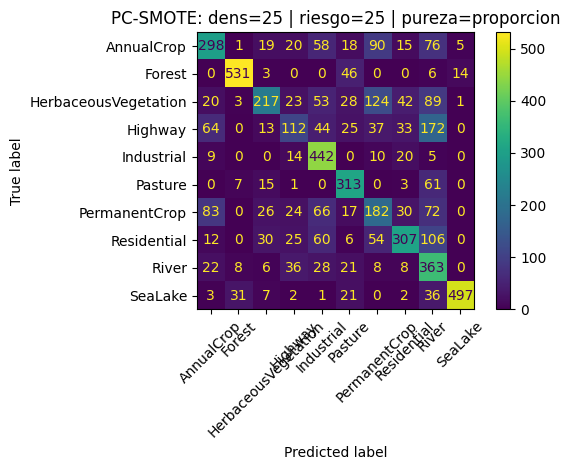
\includegraphics[width=0.6\textwidth]{pcsmote_heatmap_best.png}
  \caption{Matriz de confusión para la mejor configuración de PC-SMOTE (densidad=25, riesgo=25, pureza=proporción)}
  \label{fig:pcsmote_best_heatmap}
\end{figure}

\begin{figure}[H]
  \centering
  \includegraphics[width=0.6\textwidth]{proyeccion_3d_sinteticos.png}
  \caption{Visualización 3D del espacio generado por PC-SMOTE}
  \label{fig:proyeccion_3d_sinteticos}
\end{figure}
